\documentclass[11pt]{article}

% ==== Paquetes ====
\usepackage[utf8]{inputenc}
\usepackage[spanish]{babel}
\usepackage{amsmath, amssymb, amsfonts, siunitx}
\usepackage{graphicx}
\usepackage{float}
\usepackage{listings} % Para código
\usepackage{xcolor}
\usepackage{hyperref}
\usepackage{caption}
\usepackage{subcaption}
\usepackage{geometry}
\usepackage{tikz}

\geometry{margin=2.5cm}

% ==== Configuración de listings (para código) ====
\lstset{
  basicstyle=\ttfamily\small,
  numbers=left,
  numberstyle=\tiny,
  stepnumber=1,
  numbersep=5pt,
  backgroundcolor=\color{gray!10},
  frame=single,
  tabsize=2,
  breaklines=true,
  showstringspaces=false,
  keywordstyle=\color{blue},
  commentstyle=\color{green!50!black},
  stringstyle=\color{red!70!black}
}

% ==== Datos de la tarea ====
\title{IEE3682 - Electro-óptica \\
Tarea 2}
\author{Nicolás Seguel}
\date{Septiembre 2025}

\begin{document}
\maketitle

% ==== Ejemplo de respuesta con texto y fórmulas ====
\section*{Pregunta 1}

Se asume una onda plana con dirección de propagación z y el campo eléctrico tiene componentes \textbf{x} e \textbf{y}. Bajo estas condiciones se tiene que la ecuación de onda es:

\begin{equation*}
    E(z, t) = \Re \left\{\textbf{E}_0 e^{-j(k z - \omega t)}\right\}
\end{equation*}

El vector $\textbf{E}_0$ corresponde al campo eléctrico y para la polarización circular derecha es igual a:

\begin{equation*}
    \textbf{E}_0 = \frac{E_0}{\sqrt{2}} (\hat{x} + j \hat{y})
\end{equation*}

Ahora bien, para la polarización circular izquierda:

\begin{equation*}
    \textbf{E}_1 = \frac{E_1}{\sqrt{2}} (\hat{x} - j \hat{y})
\end{equation*}

Reemplazando estos valores de $\textbf{E}_0$ en la ecuación de onda se tiene:

\begin{align*}
    E_x(z, t) &= \frac{E_0}{\sqrt{2}} \cos(k z-\omega t) \\
    E_y(z, t) &= \frac{E_0}{\sqrt{2}} \sin(k z-\omega t) \\
    E_z(z, t) &= 0
\end{align*}

Para una onda circular izquierda es idéntico, expecto por un cambio de signo en la componente \textbf{y}. Ahora bien, si las ondas se superponen se obtiene lo siguiente.

\begin{align*}
    E_x(z, t) &= \frac{E_0 + E_1}{\sqrt{2}} \cos(k z-\omega t) \\
    E_y(z, t) &= \frac{E_0 - E_1}{\sqrt{2}} \sin(k z-\omega t) \\
    E_z(z, t) &= 0
\end{align*}

Donde $E_0$ corresponde a la amplitud de la polarización circular derecha y $E_1$ corresponde a la amplitud de la polarización circular izquierda. Es importante notar que tenemos distintos casos dependiendo de la amplitud de cada polarización. Primero, si $E_0 = 0$ o $E_1 = 0$, se tiene polarización circular derecha o izquierda, respectivamente. Segundo, si $E_0 = E_1$ se cancela la componente en \textbf{y}, quedando solo las variaciones en la componente \textbf{x}, por lo que se tiene una polarización lineal. Por ultimo, cualquier valor intermedio implica que la amplitud de la componente \textbf{y} es menor a la componente \textbf{x}. Esta diferencia en la amplitud de las componentes implica que el campo eléctrico tiene una polarización elíptica.

En la figura \ref{fig:pol_elip} se muestra una simulación en GeoGebra que muestra la superposición de dos vectores que siguen una trayectoria circular y su suma, que sigue una trayectoria elíptica.

\begin{figure}[H]
    \centering
    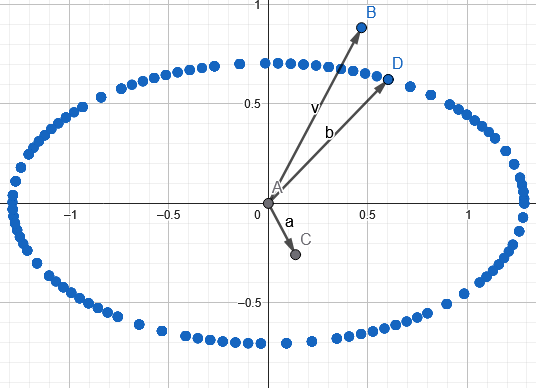
\includegraphics[width= 0.8\linewidth]{pol_elip.png}
    \caption{Simulación vectorial de los campos para polarización elíptica.}
    \label{fig:pol_elip}
\end{figure}

\section*{Pregunta 2}

\subsection*{a.}

Aplicando a la transformada de Fourier a la función $g(z, t)$ se tiene que:

\begin{equation*}
    G(k, \omega) = \int_{\infty}^{-\infty} \left[\int_{\infty}^{-\infty} g(z, t) e^{-j k z} \,dz \right] e^{-j \omega t} \,dt
\end{equation*}

De esta ecuación es claro ver que las bases de Fourier son independientes entre sí, por lo que se puede escribir la transformada 2D de Fourier como:

\begin{equation*}
    G(k, \omega) = \iint_{\infty}^{-\infty} g(z, t) e^{-j k z} e^{-j \omega t} \,dz \,dt
\end{equation*}

La transformada inversa se puede escribir como:

\begin{equation*}
    \boxed{g(z, t) = \frac{1}{4 \pi^2}\iint_{\infty}^{-\infty} G(k, \omega) e^{j k z} e^{j \omega t}\,dz \,dt}
\end{equation*}

que corresponde a una superposición de armónicos de $e^{j (k z + \omega t)}$.

\subsection*{b.}

\subsection*{c.}

\subsection*{d.}

\subsection*{e.}

\section*{Pregunta 3}

\subsection*{a.}

\subsection*{b.}

\section*{Pregunta 4}

\subsection*{a.}

\subsection*{b.}

\subsection*{c.}

\subsection*{d.}

\subsection*{e.}

\subsection*{f.}

\end{document}
